\documentclass{article}
\usepackage{doc,url,verbatim,fancyvrb}
\usepackage{pifont}
\usepackage[authoryear]{natbib}
\usepackage[pdftex]{graphicx}
\usepackage{gretl}
\usepackage{hyperref}
\usepackage[letterpaper,body={6.3in,9.15in},top=.8in,left=1.1in]{geometry}

\setlength{\parindent}{0pt}
\setlength{\parskip}{1ex}

\title{geoplot: cartography in gretl}
\author{Allin Cottrell and Jack Lucchetti}

\begin{document}

\maketitle

\textbf{Warning}: As of this writing the \textsf{geoplot} package is
in ``alpha'' mode (or at best ``beta''). You're welcome to try it, but
expect some bugs, and do not bank on the user interface remaining
unchanged.

\section{Preliminaries}
\label{sec:prelim}

Given gretl's user base and vocation, we assume that people will be
primarily interested in ``thematic'' maps, in which geographical areas
get different colors according to some variable of interest (for
example regions of a country are colored according to their
unemployment rates). Fancier maps are out of scope for the
present. From here on we'll simply refer to maps of this sort as
``maps'' and the geographical entities they contain as
``regions''. Plotting a map typically involves drawing a number of
polygons, filled with appropriate colors, to some device (the screen,
or a file).\footnote{One may want to draw colored lines, such as
  rivers or roads. Probably doable, but not for now.}

The essential ingredients for doing this are
\begin{enumerate}
   \item A geometrical description of the regions.
   \item The data for coloring the polygons.
   \item Appropriate software for producing the map. 
\end{enumerate}
   
\subsection{The geometry}
\label{sec:geometry}

Let's say we have $n$ regions, indexed by $i$. Each region $i$ is
represented geometrically as a collection of $k_i$ polygons (think
islands in an archipelago), indexed by $j$. Each polygon is defined by
$h_{i,j}$ coordinates. Typically, each coordinate vector has two
elements, latitude and longitude.\footnote{In some cases you may have
  a third element---altitude being the most obvious candidate---or
  more.  But we're not getting into that right now.}

The information on each region comprises two components:
\begin{description}
\item[Metadata] At minimum this should include the region's
  identifier(s), as a string and/or numerical codes. Other
  information, such as land area, may also be included. You can see
  this as a dataset with $n$ observations and several variables,
  possibly string-valued.
\item[Polygon data] A geometrical representation of a region's shape
  on the map, in the form of one or more polygons, each represented by
  an array of X--Y pairs, typically latitude and longitude. You can
  see this as an array of arrays of 2-column matrices: the outer array
  is of size $n$; the inner arrays each contain $k_i$ matrices, each
  with two columns.
\end{description}

Several file formats can be used for storing the geometry information.
The page
\url{https://ec.europa.eu/eurostat/web/gisco/geodata/reference-data/administrative-units-statistical-units/nuts}
contains a nice collection for European NUTS regions (NUTS =
Nomenclature of Territorial Units for Statistics).  The
\textsf{geoplot} package supports two formats:
\begin{enumerate}
\item GeoJSON files: plain JSON files with a
  pre-specified internal structure, regulated by RFC 7496. Basically,
  an array of regions (or ``features'') with each element containing
  the metadata and the polygons, under the \texttt{properties} and
  \texttt{geometry} keys, respectively.  This is our preferred format.
\item ESRI shapefiles: more of a ``legacy'' format, but still very
  common in the wild. These maps come as collections of several files,
  the essential ones being:
  \begin{itemize}
  \item an xBase file, with \texttt{dbf} extension, holding the
    metadata;
  \item the shapefile proper, with a \texttt{shp} extension, holding the
    polygons;
  \item an index file, with a \texttt{shx} extension, used to speed up
    operations when you read the data.
  \end{itemize}
\end{enumerate}

In the future we may take a look at an evolution of GeoJSON called
TopoJSON, but that's not a priority at the moment.

\subsection{The payload}
\label{sec:payload}

The data for coloring the polygons constitute what we call the
``payload''. We assume that the user has the payload data as a gretl
series; typically, but not necessarily, this means that the user has a
datafile (in \texttt{gdt} or CSV format) where each line represented a
region, as in Table~\ref{tab:payload}. Note the \texttt{id} column: it
is assumed that the map metadata contain some information to establish
a correspondence with the dataset containing the payload series.
Ideally this should be a numerical code, but a string-valued variable
is also be acceptable.


\begin{table}[htbp]
\begin{center}
\begin{tabular}{lrrr}
  \hline
  \textbf{id}	& \textbf{State}& \textbf{Pop2019} & \textbf{Pop2010} \\
  \hline
  1	& Alabama	& 4903185	& 4779736  \\ 
  2     & Alaska	& 731545	& 710231   \\ 
  101   & American Samoa	& 55641	& 55519	  \\ 
  3	& Arizona	& 6278717	& 6392017  \\ 
  4	& Arkansas	& 3017825	& 2915918  \\ 
  5	& California	& 39512223	& 37254523 \\ 
  6	& Colorado	& 5758736	& 5029196  \\ 
  7	& Connecticut	& 3565287	& 3574097  \\
                & \vdots & \\
  \hline
\end{tabular}
\end{center}
\caption{Typical format for the payload data}
\label{tab:payload}
\end{table}


\subsection{The software backend}
\label{sec:software}

One could conceivably use any one of the many plotting libraries
around, but the \textsf{geoplot} package uses \textsf{gnuplot}, which
is already used for all other kinds of plot in gretl.  The gnuplot way
of drawing maps is via the Swiss-army knife \cmd{plot} command, with
the \texttt{filledcurves} style. Details on the gnuplot syntax we're
using are in Appendix \ref{sec:gnuplot}.

Given the geometry data and the payload, writing a gnuplot script for
producing the map is relatively straightforward. The only possible
problem could be its size for maps with lots of regions.

\section{The workflow}
\label{sec:workflow}

Given the above, we could organize the workflow for having a map
plotted in gretl as follows:

\begin{enumerate}
\item you \cmd{open} the map-datafile into an ordinary dataset; this
  will read the metadata so \dollar{nobs} will be equal to $n$.
\item you create the payload series via append/join/whatever;
\item you decide on the details of your map (color scale, possibly
  add points/lines, send it to a png file or view it, etc), with
  sensible defaults;
\item finally, you create the map. 
\end{enumerate}

Point 1 is handled by using the existing "open" command on the
map-datafile (a GeoJSON file or a dbf file for the ESRI
format).\footnote{It would be desirable to be able to \cmd{store}
  GeoJSON files too, but we'd need a fast and efficient way to write
  JSON files. At this time, Artur's function in the \texttt{extra}
  package is not fit for the purpose because we need to store arrays
  of arrays.} In principle, we could read the the geometry data at
this point and store them in RAM, but (at least for now) we don't, to
avoid filling up the RAM with lots of polygons. Instead, we read the
metadata \emph{only} and the link with the geometry data is provided
by storing the location of the geometry file internally; possibly, we
could provide an accessor (\dollar{mapdata}?)  to let the user know if
necessary.\footnote{Internally, this will most likely be handled by
  using CSV as an intermediate format, but all this will be completely
  transparent to the end user.} If we change our mind about this, the
\dollar{mapdata} accessor will probably point to a structure with the
geometry data: the internal representation of the geometry we have now
when we read from the GeoJSON format is an array of bundles, one per
region.

For point 2 we need no additional work. As for points 3) and 4), a
possibility is a "command-block" approach, where these two actions are
coalesced into a "geoplot" block, similar in syntax to the existing
\cmd{plot} command.

\begin{scode}
  open lad.json 
  series x = normal() 
  geomap x 
     options <whatever> 
  end geomap --output=display
\end{scode}

Note that \cmd{geomap} would read from the ``hidden'' geometry
file. In principle, we may gain some additional flexibility by reading
the geometry into a bundle array at point 1, but while it's
straightforward to get such an object from JSON, it's not so easy
(though clearly feasible) to construct one from a .shp file. Besides,
most users will just want to add a data series, pick some options for
how the map should look, and generate a map-image.  And for that we
don't need to hold a heavyweight object (all those polygons) in
memory.

Some expert users might want to mess with the bundle
representation of the full map data as such, but an expert function to
retrieve it could be added.

The \cmd{geomap} command would take care of (a) reading in the
geometry file (the GeoJSON file again, pairing the polygon data with
the payload series (there may be a few problems here: see section
\ref{sec:pairing}) and shipping the result to gnuplot, possibly with
graphical refinements, as dictated by the options inside the block.

At the time of writing, we don't have yet everything implemented in
libgretl, so in hansl we have to make do with alternative
solutions. In the \texttt{geoplot.gfn} package, we have a few hansl
functions for manipulating map data, that we can use for producing
simple examples and prototyping the algorithms.

\section{An example}
\label{sec:example}

For this example, we'll produce a map with the GDP per capita of the
6 founder countries of the EU and use 3 files: \texttt{founders.inp},
\texttt{founders.csv} and \texttt{founders.geojson}. This has the
advantage that the necessary files are small enough to be inspected by
hand if necessary.  The contents of the \texttt{founders.csv} file,
that contains the eventual payload, are
\begin{code}
Name,code,pop,area,gdp
Belgium,BE,11365834,30528,534230
France,FR,67024633,632833,2833687
Germany,DE,82437641,357386,3874437
Italy,IT,61219113,301338,2147744
Luxembourg,LU,589370,2586.4,65683
Netherlands,NL,17220721,41543,880716
\end{code}
\begin{table}[htbp]
  \hrulefill
  \begin{scriptsize}
  \begin{code}
{"type": "FeatureCollection", "features": [
 {"geometry": {"type": "Polygon", "coordinates": [[[40.40360,
     30.79039], [40.59686, 30.49366], [40.65087, 30.29746], ... ]]},
   "type": "Feature", "properties": {"CNTR_NAME": "Belgique",
     "ISO3_CODE": "BEL", "CNTR_ID": "BE", "NAME_ENGL": "Belgium",
     "FID": "BE"}, "id": "BE"},
 {"geometry": {"type": "MultiPolygon", "coordinates": [[[[40.18497,
     29.45664], [40.23634, 29.39875], [40.57754, 29.35021], ...],
     [[[42.66689, 20.70300], [42.57348, 20.41660], ...]]},
   "type": "Feature", "properties": {"CNTR_NAME": "France",
     "ISO3_CODE": "FRA", "CNTR_ID": "FR", "NAME_ENGL": "France",
     "FID": "FR"}, "id": "FR"},
  ...
\end{code}
  \end{scriptsize}
\hrulefill
\caption{Excerpt of \texttt{founders.geojson}}
\label{tab:json-xrpt}

\end{table}
The JSON file is too large to be shown here in full, but it's small
enough that any text editor will do; Table \ref{tab:json-xrpt}
contains a significant excerpt. Note that Belgium is a single polygon,
but France is a collection of polygons, because of Corsica.

\begin{table}[htbp]
\begin{scode}
set verbose off
include geoplot.gfn
mapfile = "founders.geojson"
open "@mapfile" --preserve

join founders.csv gdp pop --ikey=FID --okey=code
series gdppc = 1000*gdp/pop

opts = defbundle("plotfile", "GDPpc.gp", "inlined", 1)
geoplot(mapfile, gdppc, opts)
\end{scode}
\caption{The ``founders'' script}
\label{tab:founders-script}
\end{table}

The \texttt{founders.inp} script is in Table
\ref{tab:founders-script}; the only reason why we use the
\option{preserve} option when we \cmd{open} the GeoJSON file is to
keep track of the string with the filename, but this will go
eventually; this is what we get after opening the json file:
\begin{code}
     CNTR_NAME    ISO3_CODE      CNTR_ID    NAME_ENGL          FID

1     Belgique          BEL           BE      Belgium           BE
2       France          FRA           FR       France           FR
3  Deutschland          DEU           DE      Germany           DE
4       Italia          ITA           IT        Italy           IT
5    Luxemburg          LUX           LU   Luxembourg           LU
6    Nederland          NLD           NL  Netherlands           NL
\end{code}

Next, we perform the \cmd{join} with \texttt{FID} (from the JSON file)
as the inner key and \texttt{code} (from the CSV file) as the outer
key. Finally, since we don't have the \cmd{geomap} block yet, for now
we use a \cmd{geoplot} function, whose signature is
\begin{code}
function void geoplot(const string mapfile,
	const series payload[null],
	const bundle options[null])
\end{code}
where \texttt{mapfile} is the filename of the file containing the
outlines, \texttt{payload} is the (optional) series with which to
colorize the polygons, and \texttt{options} is a bundle to contain one
or more optional elements governing the appearance of the
plot.\footnote{We're using a bundle to allow an arbitrary number of
  options without over-burdening the signature of the function.}

If the \cmd{geoplot} call in fact follows on the opening of a map
metadata file in the same session, the mapfile argument may be
regarded as already implicit (it will be the very same file in the
GeoJSON case, or an shp file with the same basename as a previously
opened dbf file), but for now we're requiring that its path be
given.

If the payload is \texttt{null} or omitted, then only the
boundaries between region will be drawn, so the user can inspect the
outlines without any colorization, in case that could be useful.  this
is useful if you want to have a see what a geometry file looks like.

If the \texttt{options} bundle is omitted all options are set to their
default values. The list of keys that are currently handled in the
options bundle is listed in section \ref{sec:opts}. Here, we just use
two: the ``plotfile'' option is used to store the generated gnuplot
script into the \texttt{GDPpc.gp} file; moreover, this file will
contained the geometry data in ``inlined'' form.

Running the script will produce a gnuplot file like the following:

\begin{code}
set term wxt persist

unset key
set cbrange [33.3288:117.018]
set xrange [31.7826:51.4213]
set yrange [14.7701:36.0553]
$MapData << EOD
40.4036 30.79039 47.00315
40.59686 30.49366 47.00315

[...]

38.92268 31.40258 51.142806
38.59809 31.50169 51.142806
38.59737 31.60855 51.142806


EOD
plot for [i=0:*] $MapData index i with filledcurves fc palette, \
  $MapData using 1:2 with lines lc "white" lw 1
  
\end{code}
%$

and feeding the above into gnuplot will yield  this map:

\begin{center}
  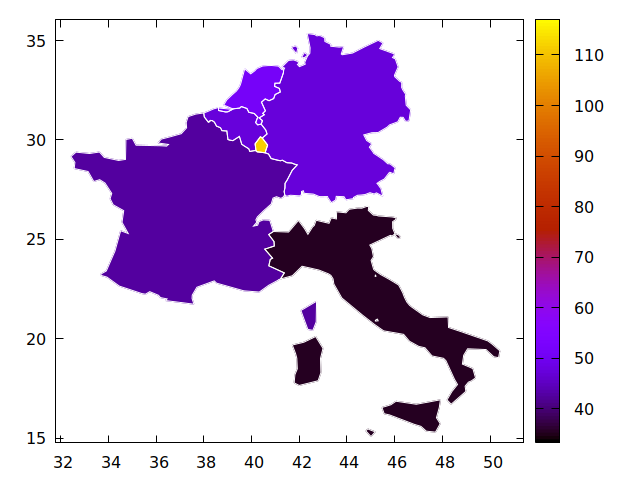
\includegraphics[scale=0.5]{GDPpc.png}
\end{center}

\subsection{The pairing problem}
\label{sec:pairing}

The strategy outlined above implies a possible problem, arising from
the decoupling of the metadata and the geometry data that takes place
when you \cmd{open} the former.

\begin{table}[htbp]
  \begin{scode}
set verbose on
include geoplot.gfn

open "us-states.geojson" --quiet

x = normal()
opts = defbundle("plotfile", "us0.gp", "inlined", 1, "show", 1)

opts.title = "USA (complete)"
geoplot("us-states.geojson", x, opts)

# now suppose you don't want Alaska and Hawaii

series dum = (abbrev != "Alaska") && (abbrev != "Hawaii")
x = dum ? x : NA
opts.title = "USA (mainland)"
opts.plotfile = "us1.gp"
geoplot("us-states.geojson", x, opts)
  \end{scode}
  \caption{US maps (complete vs mainland)}
  \label{tab:USA}
\end{table}

In order to proceed with the creation of the map, it is tacitly
assumed that a 1:1 correspondence between the $n$ regions one has in
the currently open dataset and those in the geometry file can be
established.

\begin{figure}[htbp]
  \begin{center}
  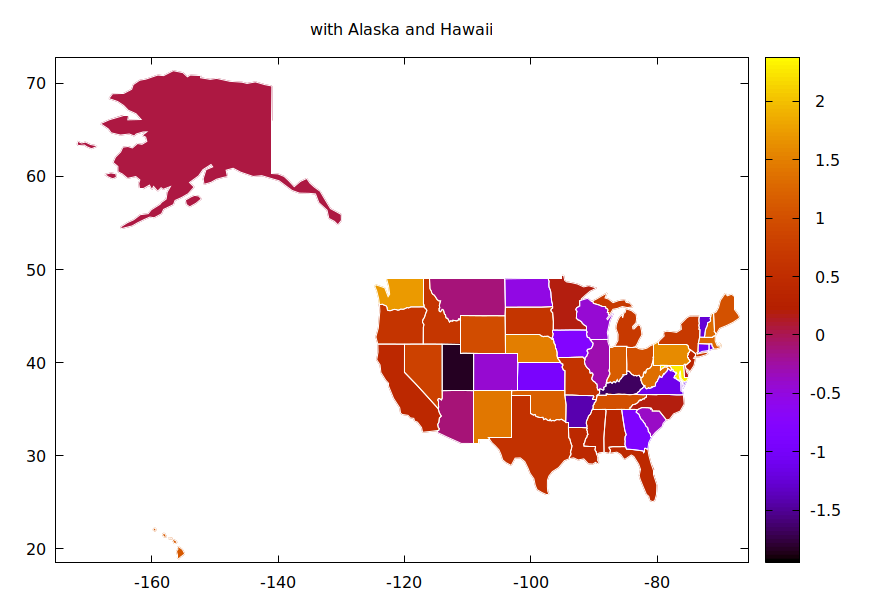
\includegraphics[height=180pt]{us0.png}

  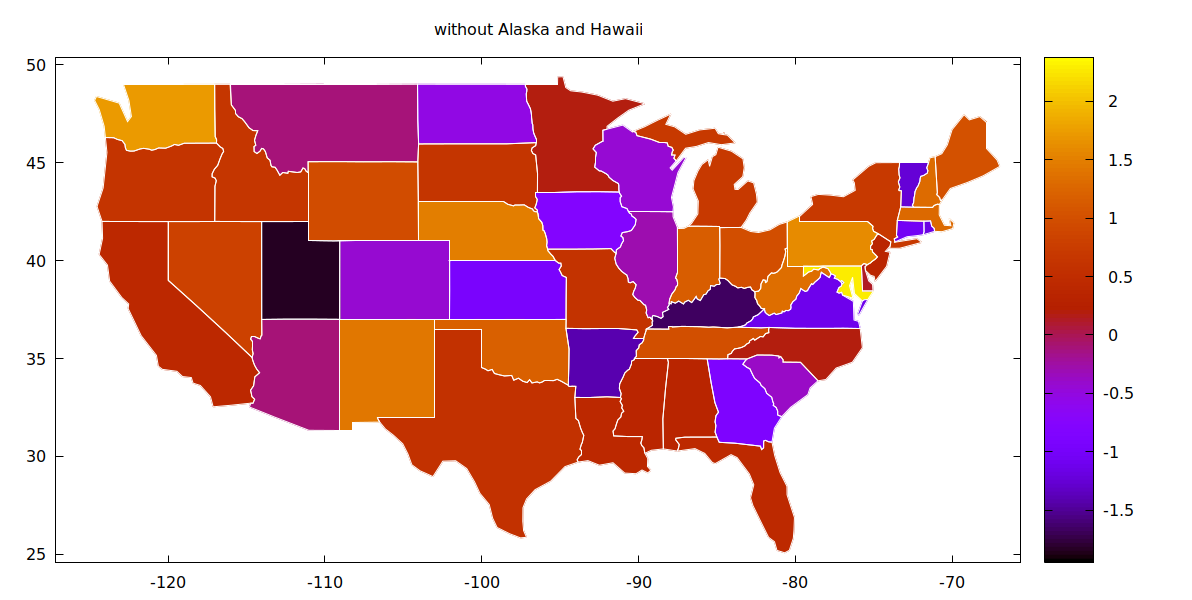
\includegraphics[height=180pt]{us1.png}  
\end{center}
\caption{Output of script \ref{tab:USA}: full US vs mainland only.}
\label{fig:USA}
\end{figure}

Two possibilities (are there any more?) when this correspondence may
be broken are: (i) sorting and (ii) subsampling. In both cases,
observation $i$ in the currently open dataset wouldn't correspond with
the $i$-the region in the geometry datafile. Sorting is a relatively
unusual operation, but subsampling is arguably very important, because
in many cases one wants to produce maps that show only a subset of the
available regions. A typical case is the USA, where you often want to
leave out Hawaii, and possibly Alaska too.

The solution we have for the moment for subsampling is to ``fake''
subsampling by stuffing \texttt{NA}s into the payload: see for example
the \texttt{US.inp} script shown in table
\ref{tab:USA},\footnote{Given the nature of the example, we don't pick
  up the payload from a file, but just generate it via
  \texttt{normal()}.}  that produces the maps shown in Figure
\ref{fig:USA}. This works, but feels like a bit of a hack and we'll
have to think of a way to handle this more gracefully.

A related, but different problem arises when the map data and the
payload come from different sources. In this case, there may be a
problem of \texttt{join}ing the regions correctly if discrepancies
arise between the inner and outer keys. But this is not a problem of
the mapping apparatus, bit rather a more general issue on matching
data from different sources, and we need not be concerned with it
here.

If the \cmd{geoplot} function is invoked without a payload, so to just
draw the boundaries between regions, one can use the \texttt{mask} key
of the options bundle to indicate which regions must be skipped.

\clearpage
\appendix

\section{Representation of polygons in gnuplot}
\label{sec:gnuplot}

The
following \texttt{gnuplot} code
\begin{code}
  unset key
  plot '-' using 1:2:3 with filledcurves fillcolor "blue"
  0 0 0
  0.5 0 0.866
  1 0 0
  e
\end{code}
produces an equilateral triangle: 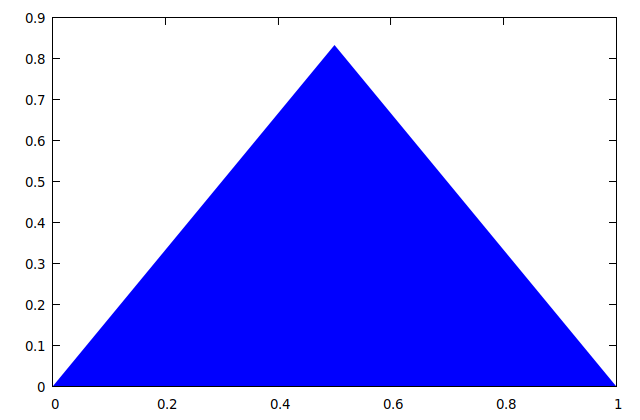
\includegraphics[height=2cm]{triangle.png}

\medskip

The internal coloring of each polygon can be set by using the
\texttt{fillcolor palette} syntax. For example,
\begin{scriptsize}
\begin{code}
unset key
plot for [i=0:*] '-' index i with filledcurves fillcolor palette
	0 0 2.5 
	0 1 2.5
	1 1 2.5
	1 0 2.5

	2 1 3.5 
	2 2 3.5
	3 2 3.5
	3 1 3.5

	4 0 3 
	4 1 3
	5 1 3
	5 0 3

e
e
e        
\end{code}
\end{scriptsize}
produces
\begin{center}
  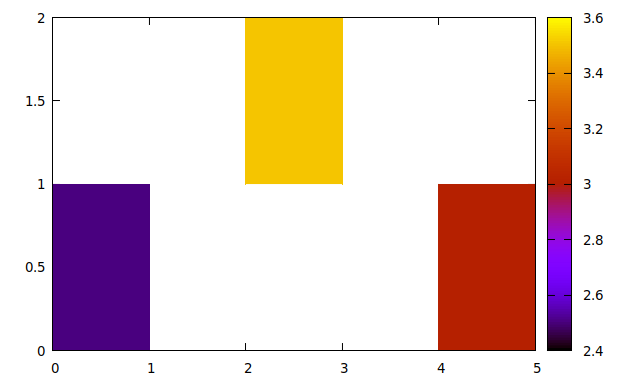
\includegraphics[width=0.8\textwidth]{squares}
\end{center}

A nice way to customize the palette is by using the syntax \texttt{set
palette defined} (see the gnuplot manual).

\section{Currently supported options for the \texttt{geoplot} function
(in alphabetical order)}
\label{sec:opts}

Note that the options we have now don't form a fully coherent set: for
example, the \texttt{plotfile} key is useless when \texttt{show} equal
1, but we have time to optimize that.

\begin{description}
\item[\textbf{bordwidth}:] scalar, thickness of the line used for the
  borders: Default: 1.
\item[\textbf{datfile}:] filename, allowing the user to direct output
  of the representation of the polygon data for use with
  gnuplot. Default: \texttt{geoplot\_tmp.dat} in the user’s
  \texttt{dotdir}.
\item[\textbf{height}:] scalar, giving the height of the plot (in
  pixels for PNG output, which is the only case handled so far). If
  this is given we try to figure out the width which gives a suitable
  aspect ratio for the plot and write these dimensions into the plot
  file. Default: no dimensions written into the plot file; you get the
  whatever is the gnuplot default.
\item[\textbf{inlined}:] Boolean, to have the polygon data included
  directly into the gnuplot file. Default: the data are read from a
  separate file (see datfile).
\item[\textbf{logscale}:] Boolean, logscale for the payload. Default: false.
\item[\textbf{mask}:] a column vector of length equal to the number of
  features in the map, with zeros in all places other than features to
  be excluded, which should be represented by \texttt{NA}s. This is
  very much a provisional formulation and should be improved. The mask
  is referenced only if payload is not provided; it provides an
  alternative means of sub-setting the features. Default: none.
\item[\textbf{notics}:] Boolean, for turning off the printing of x
  (longitude) and y (latitude) tics. Default: tics are printed.
\item[\textbf{plotfile}:] filename, allowing the user to direct output
  of the generated gnuplot command file. Default: geoplot.gp in the
  user’s working directory.
\item[\textbf{setpal}:] string, giving a gnuplot set palette command,
  to be injected into the plot file. For example, the syntax
  \begin{code}
    options.setpal = "set palette defined (0 '#D4E4F2', 1 'steelblue')"  
  \end{code}
  will give you a pleasent blue gradient.  Default: the standard
  built-in gnuplot palette (nothing extra is written into the plot
  file).
\item[\textbf{show}:] Boolean, specifying if the plot should be shown
  on-screen right away. Default: true. (Otherwise a gnuplot file is
  written but not displayed.)
\item[\textbf{title}:] string specifying a title for the
  plot. Default: no title.
\end{description}

\end{document}

%%% Local Variables:
%%% mode: latex
%%% TeX-master: t
%%% End:
